\documentclass[a4paper,11pt]{report}
\usepackage[T1]{fontenc}
\usepackage[utf8]{inputenc}
\usepackage{lmodern}
\usepackage{graphicx}
\usepackage{eurosym}
\usepackage{fancyhdr}
\pagestyle{fancy}
\lhead{Hack Cyprus}
\rhead{Hackathon proposal}

\begin{document}

\begin{titlepage}
\begin{center}
% Upper part of the page
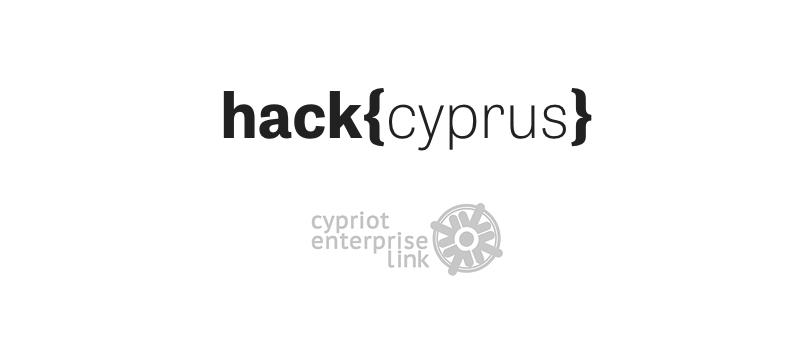
\includegraphics[height=5cm, width=0.9\textwidth]{cel}\\[1cm]    
% Title
{ \huge \bfseries Hack Cyprus 2012 Proposal}\\[0.4cm]
% Author and supervisor
\begin{minipage}{0.4\textwidth}
\begin{flushleft} \large
\emph{Author:}\\
Cypriot Enterprise Link
\end{flushleft}
\end{minipage}
\begin{minipage}{0.4\textwidth}
\begin{flushright} \large
\emph{Date:} \\
25 July, 2012
\end{flushright}
\end{minipage}
\vfill
% Bottom of the page
{\large \today}
\end{center}
\end{titlepage}



\tableofcontents
%Chapter 1
\chapter{Hack Cyprus 2012}
\section{Introduction}
A hackathon is an event destined to bring software developers, graphic designers and ideators together. A hackathon typically lasts 2-3 days (usually over a weekend) and the participants work intensely in teams, in order to develop new ideas. At the end of a hackathon there is a series of demonstrations in which each team demonstrates its work and a panel of judges (or the other participants) decides which the winning teams are.

A common misconception is that a hackathon is related to malicious operations on software systems. However, this is just a misconception and according to the HackDay Foundation \footnote{http://hackday.co/about}, although “hack” is in the root of hackathon, hackathons have nothing to do with malicious “hacking” done by crackers, rather the spirit of a hackathon is to collaboratively build programs and applications.

The ideas developed at a hackathon vary from simple web or smart phone applications to sophisticated websites and even hardware applications. The main difference between a hackathon and a normal competition is that prototypes of these ideas must be developed in less than 48 hours and usually they must be commercially viable products (although this is not a requirement).  

Therefore, in the spirit of the hackathon culture described above, we decided to organise our own hackathon which will be the \textbf{first ever weekend-long hackathon in Cyprus}. The name of the event is Hack Cyprus 2012 and it's official website is \textbf{http://hackcyprus.com}.

\section{Objectives}
The objectives of Hack Cyprus 2012 are tied to the objectives of the Hack Cyprus initiative, discussed later in this proposal. Our main goal is to connect like-minded people and create an event where synergies between young Cypriots will be created. We believe that when people join forces they can achieve amazing things. A hackathon is probably one of the best ways to achieve this. 

Another important goal is to help and inspire young Cypriots to pursue their dreams and exercise their skills. We are aware that a large proportion of young Cypriots are unemployed, even though most of them are highly educated and have the skills to succeed. Our hackathon will encourage young Cypriots to take action, develop their ideas and at the same time meet other people who share a common vision. 

\section{Logistics}
\subsection{Event date}
The event will take place over the first weekend (1/9 - 2/9) of September. The rationale behind this decision is twofold:
\begin{enumerate}
  \item September follows the summer holidays and everyone is getting back into their work routine.
  \item Most of the students studying abroad will still be in Cyprus by then.
\end{enumerate}
\subsection{Expected attendance}
The expected attendance is 40-50 people. This number is based on the support (120 people) we have received so far on our landing page.
\subsection{Venue location}
We are currently discussing with several venue providers regarding the location and the venue of the hackathon, TEPAK and UCY being amongst them. The venue is required to provide high-speed Internet connection, sufficient space for the teams to work comfortably and the basic infrastructure to support the electrical and electronic devices (e.g laptops and monitors) that the participants will be using during the hackathon. Ideally, the venue should be available to us overnight since the spirit of the hackathon dictates that the teams should be able to work all day long without any disruption. 
 
\section{Theme}
Usually, teams are free to select what they will work on but occasionally hackathons can have a theme such as a ''green'' or ''music'' hackathon, where the participants must develop applications related to the environment or music respectively. For Hack Cyprus 2012 we have decided to allow each team to develop its own idea without any restriction on the theme. The reason for this is due to the fact that this event is the first of its kind in Cyprus and a themed hackathon would decrease the number of participants significantly. 

\section{Target group}
By definition a hackathon is open to coders, designers, ideators and entrepreneurs. Ideally, a team participating in our hackathon will
be comprised of a combination of these types of people. From our experience with hackathons in the UK and the US, the participants will be mostly males in the age range 18 to 40 years old.   

\section{Mentors}
Mentors are an integral part of any hackathon. They can be experienced programmers, entrepreneurs or university professors and their responsibilities cover a wide range. More specifically, our mentors will serve three main purposes:
\begin{enumerate}
  \item \textbf{Mentors to the teams}: Technical minds to guide and assist the given teams with any technical requests or help they might have, in a way that will not place one team into a more competitive position than others or jeopardize anyone else’s efforts. This kind of mentors should   be at equal or comparable levels to the skills and assets of the team members they will accompany.
  \item \textbf{Judging panel}: At the conclusion of the Hack Cyprus 2012, the developed prototypes will then be judged by the expert judging panel.
  \item \textbf{Presentations/story sharing}: We want to inspire our participants and give them the opportunity to hear from experienced people in the industry how they managed to overcome the barriers and march to success. 
\end{enumerate}

\section{Winning team selection criteria}
Since our hackathon is open to any kind of technology-related ideas it is extremely difficult to set objective criteria for the selection of the winning idea. However, similarly to hackathons organised in other countries, we can use a set of subjective criteria to select the winner. Given that the judges will be experienced in the fields of technology, business development and innovation these criteria will suffice to ensure that the teams will be judged on a fair basis.

The criteria we have set are:
\begin{enumerate}
  \item Originality of idea
  \item Quality of implementation (Did they develop a working demo?) 
  \item Market Potential (Does this idea appeal to a large demographic or is it a niche app?)
  \item Teamwork (did they demonstrate teamwork spirit and work together effectively?)
\end{enumerate}

\section{Sponsors}
Hackathons are events that do not require large amounts of money to be organised since they can be easily bootstrapped. However, if the organisers wish to take the hackathon a step further by attracting high-profile people and develop high quality ideas a substantial amount of funding is needed. This is exactly what our team wishes to achieve but at the same time we are determined to keep the costs at a minimum. 
 
\subsection{Food and drinks}
A hackathon is about developing and hacking away ideas in a very short amount of time and the organisers should ensure that participants work under the best possible conditions. We aim to achieve this by ensuring that there will be enough food and beverages for the contestants, always free of charge. We have assembled a list of potential food and drinks sponsors and our team is currently trying to get them on board.  

\subsection{Prizes}
Hack Cyprus 2012 is a competition and we want to ensure that the hard work of the participants will be recognised. For this reason, potential prizes sponsors have been contacted by members of our team. 

\section{Provisional schedule}
Hack Cyprus 2012 will be a weekend-long hackathon which means that the teams will have more than 24 hours to develop their ideas. The provisional schedule of the event is shown below. \\

\noindent\textbf{Saturday:}\\
9:30 Event starts - registration - coffee - snacks - networking\\
10:30 Organizers - mentors - aim - prizes\\
11:00 Brief talks by sponsors\\
11:30 Pitching\\
12:00 Team formation - hacking starts\\
14:00 Lunch\\
21:00 Dinner\\

\noindent\textbf{Sunday:}\\
9:30 Breakfast \\
14:00 Lunch\\
17:00 Hacking stops - teams prepare presentations\\
17:30 Presentations \\
18:00 Prizes\\

Additionally, during the hackathon we will have brief talks by our sponsors or mentors. Furthermore, based on the feedback we have receibed from potential attendees we decided to include in the schedule brief talks where attendees can present something they have built and they want to showcase it.

\section{Provisional budget}
\begin{table}[h]
\caption{Provisional budget based on 50 attendees} %title of the table
\centering % centering table
\begin{tabular}{l c} % creating eight columns
\hline\hline                        %inserting double-line
Expense & Amount \\ [0.5ex]   
\hline            
Food and drinks  & 1500 euro\\ % Entering row contents
Prizes           & 800 euro\\
Marketing        & 500 euro\\
Mentors expenses & 2400 euro\\
Cleaning         & 200 euro\\
Various small expenses (e.g. cables, routers, projector)  + contingency & 600 euro\\
\hline 
\textbf{Total} & \textbf{6000 euro}\\
\hline
\end{tabular}
\end{table}

%Chapter 2
\chapter{Who are the people behind the hackathon?}

\section{Cypriot Enterprise Link}
The Cypriot Enterprise Link (CEL) is a fresh youth-led organization aimed to connect and support the Cypriot entrepreneurial talent in order to form a local and a global entrepreneurial network supported by events, meet-ups, workshops and projects. 

CEL was created in late 2011, by Michael Tyrimos, Angelos Perdios and Michael Hadjijoseph, and was soon reinforced by a group of ambitious and talented young Cypriots, who joined the team on a volunteer basis. Our team, which now counts 10 members in Cyprus, UK and Greece, consists of students, entrepreneurs, developers and industry experts. 

As a result of our diverse team, CEL keeps close ties with universities such as Cambridge, Imperial College and Harvard, as well as similar initiatives/organizations such as NACUE and Entrepreneur First in the UK; Start Up Live Athens in Greece; and of course TEDxNicosia and other Cyprus-based counter parts, which now form a roundtable in support of entrepreneurship in Cyprus. Our boundaries are therefore not limited to Cyprus, but extend to young talented Cypriots across the world.

Although we don’t have a legal formation yet, we are making our impact in the following ways:
\begin{enumerate}
  \item By creating synergies between Cypriot entrepreneurs, via informal meet ups and networking sessions, which have so far launched in Cyprus, the UK and soon in Greece. 
  \item Via our Facebook page and online communications, which led to the involvement of several individuals, who came in support of our cause.
  \item Via our planned events and topic-specific workshops (e.g: social media, intellectual property).
  \item Via our upcoming blog and featured stories on Cypriot entrepreneurs, which can inspire the efforts of others. 
\end{enumerate}

In this manner CEL attempts to raise a cultural awareness in entrepreneurship in Cyprus, thereby contributing to the construction of a wider ecosystem, comprising of angel investors, incubators and enterprise competitions. Although we are a long way from our target, we are taking consistent steps towards materializing our goal. Recent articles in the US magazine Inc (titled: Is this Paradise for Entrepreneurs?) and Cyprus Mail (titled: Growing ideas, growing business), are testament to the determination and coordination of CEL and its partners over the course of the last few months.

As part of CEL’s cultural awareness campaign, CEL will be dedicating a vast part of its dynamic on the following areas:
\begin{itemize}
  \item The Hack Cyprus initiative, for the first ever hackathon weekend in Cyprus.
  \item The Women in Entrepreneurship initiative, featuring distinguished female entrepreneurs who will share their personal stories on setting up their own businesses and giving flesh to their ideas in Cyprus.
  \item The CELLs, geo-centric network nodes of Cypriot Enterprise Link across the globe. 
\end{itemize}

We are looking for further support by established organizations and individuals that are innovative, open-minded and forward-looking in order to help us realize our goal.

\section{Hack Cyprus}
Hack Cyprus is part of the CEL initiative but it is focused on the technological aspect of the Cypriot entrepreneurial ecosystem. Similarly to many initiatives in other countries, Hack Cyprus aims to bring the tech community on the island together. The problem we try to solve is that at the moment the community seems to be fragmented and collaboration between people is either limited or non-existent. Cypriot software developers, academics, web designers and others involved in technology are scattered all over the world making collaboration and coordination almost impossible. We decided to create this initiative to enable like-minded people to share and exchange ideas related to technology and innovation and create a solid tech community on the island. 

The long-term vision of this initiative is:
\begin{itemize}
  \item Foster a community of like-minded people who love technology and innovation.
  \item Create synergies between them.
  \item Inspire young Cypriot technologists to pursue their dreams.  
\end{itemize}

One of the first steps we've taken was the creation of a Facebook group (https://www.facebook.com/groups/316689918423330/) where we invited young Cypriots who are passionate about technology to share their ideas or ask questions to be answered by fellow hackers. Initially, the group was small but soon enough it grew beyond our expectations and counts 264 members as of today. In our opinion, this proves that there is a need for a central hub for hackers to communicate and collaborate.

%Chapter 3
\chapter{Hack Cyprus and CYTA}
We strongly believe that CYTA and Hack Cyprus can build a viable partnership and cooperation in the longer term, which can be beneficial to both parties in a mutual way. Hack Cyprus will be benefit from the financial injections as well as the opportunities and guidance of CYTA. In turn CYTA will benefit in the following ways:

\begin{enumerate}
  \item The marketing actions of Hack Cyprus in a consistent and prioritized manner.
  \item Exclusive bonus events  
  \item The synergies than can manifest via a long-term cooperation.
\end{enumerate}

\section{Marketing}
As a potential sponsor and more importantly a possible and valuable strategic partner to the cause of Hack Cyprus and CEL, CYTA will receive the full attention and exposure of our marketing mix in terms of advertising, promotion and public relations. The following table explains the implementation of our proposed plan of action.

\begin{table}[h]
\centering % centering table
\begin{tabular}{l l l} % creating eight columns
\hline\hline                        %inserting double-line
Element & Details & Time frame \\ [0.5ex]   
\hline            
Advertising  & Website/Social Media                           & Entire August\\ % Entering row contents
Advertising  & Banners/mentions/leaflets                      & At the event\\
Promotion    & News letters/updates sent to members           & Mid-August – September\\
Promotion    & Sponsor’s promotional materials/gifts/prizes   & At the event\\
PR           & Interviews/publicity in various media channels & Mid-August – September\\
\hline 
\end{tabular}
\end{table}

In the next sections we will explore each of the above sections separately.

\subsection{Advertising}

To begin with, CYTA’s logos and strap lines will appear on our website under the sponsorship section, where it will accredited as an official and grand sponsor of the event. In consequence CYTA will be invited to share certain content, which is relevant to the purpose of the initiative/event and beneficial to its audience, via our social media channels. This campaign will commence throughout the entire August period and during the event, including the additional networking sections, presentations (as such) that will facilitate it.

Based on the current readings (via google analytics) our website has presented a 20\% user conversation rate within the time period of one week alone. For that very reason we are confident in the exponential growth of this ratio up to x\% by y-date, thereby accelerating the growth and maturity of our user base to reach the x-amount users. Moreover CYTA will be featured in our banners, leaflets and other content-based materials, which will circulate before and during the launch of the event, to the members of the audience, the press and any other interested parties in a physical and an electronic form.

\subsection{Promotion}

Furthermore, the sponsor and their services will be promoted extensively via tailored and dedicated features in our newsletters and updates to our user base. To add, CYTA will be invited to supply Hack Cyprus with promotional material and gifts that can be distributed amongst the attendees of the event as well as certain gifts from the “Cyta shop” that can be awarded to the winning team or section winners, under the tailored awards such as the “Cyta Prize” per se.

It should be noted that the promotion tactics in this case, will not be a stand alone effort since they will go in hand with the exposure levels that are generated from the adverting campaign; hence raising the awareness of the users and followers of the Hack Cyprus initiative in regards to CYTA, its investment in positive social change and services.

\subsection{Public Relations}

The public relations element of the marketing mix is perhaps the most important instrument at to present a more elaborative and humane picture of our sponsors, while discussing their contribution to our initiative on a national and an international level. CEL’s efforts have already been documented by CYBC, Cyprus Mail, Inc Magazine (in the US) and so forth, while the efforts of Hack Cyprus attracted the attention of the Chief Editor of TechCrunch, BBC News, Inc Magazine and other key anchors in the technology and media spectrum. Moreover, both CEL and Hack Cyprus are subject to international support by organizations such as NACUE, Start Live Up Athens and so forth, as well as local initiatives such as TEDxNicosia, Chrysallis projects and others.

Henceforth, CYTA’s positive attitude and support strategy towards the cultivation of entrepreneurship and the growth of innovation in our country will be heard loud and clear both to Cypriots and generally the techies around the world!

\section{Bonus events}
The first ever hackathon in Cyprus is designed to feature a non-restrictive theme, where any set of open ideas can be brought forward and developed by the respective teams. Further to that, CEL is planning the creation of exclusive events under the code name “Cyta Challenge” (subject to change), where the hackathon

participants will be invited to join a coding session, which will be extra to event’s standard curriculum, feature extra awards and be specific to CYTA’s demands for new applications – such as a new CYTA Vision application for example.

The given challenge will benefit CYTA via the free design and development of new applications, the increasing awareness around CYTA’s product innovation process, the presentation and implementation of new ideas that were not previously considered by CYTA’s plans.

If the process and progress of the challenge is successful, Hack Cyprus can consequently run follow up challenges on a monthly basis, and invite more of its members to review and improve the current applications. In this manner, CYTA will be brought closer to the coder community, and future customers, while receiving the expert feedback of the new generation of experts.

\section{Long-term synergies}
\subsection{Coders 2 Clients}
In addition to the above, Hack Cyprus and CEL can work together with CYTA in the longer term for the creation and growth of technology entrepreneurship zones. In other words, the members of the Hack Cyprus initiative can be invited to advice CYTA’s major customers via the VIP forum, and offer them tech based solutions to their business and operational challenges.

Such an approach will boost the trust and loyalty of CYTA’s business clients, while creating employment opportunities for the younger generation of coders. Moreover, if the given approach is successful both CYTA and CEL will be able to monitor the tangible impact and employment opportunities that were generated by their synergy. As a result Hack Cyprus will not only constitute a community of hackers, but a community of ideas that can be implemented to build solutions with an actual market valuation.

\subsection{Incubating the talent}
Considering CYTA’s vision on the creation of an incubation center, Hack Cyprus and CEL can act as a milestone in the recruitment and filtering process of the incubator’s first members, while offering guidance, content and event planning that can aid to the running and growth of the center.

Moreover, considering that Hack Cyprus has become the “Homebrew Computer Club of Cyprus” and the hotspot of the coding community in our island, it can act as the media channel for CYTA’s incubator and thereby inform and attract future members that fill the target member’s profile requirements. In this regard, the incubator will have a dedicated and related userbase, but most importantly a set, technology-oriented direction.

\section{The horizon}
To conclude, the above points showcased that our cooperation meets indeed great potential that results to win-win situation. Hack Cyprus and the hackathon do not constitute a one-off initiative or just another event, but the application of leadership to improve the existing technology standards in Cyprus and a long lasting impact with unlimited possibilities to innovate and achieve more.

\end{document}
